\chapter{Réalisation et mise en œuvre}
\begin{spacing}{1.2}
\minitoc
\thispagestyle{MyStyle}
\end{spacing}
\clearpage

\section{Introduction}

Ce chapitre présente la concrétisation de la plateforme à partir de la conception
établie précédemment. Nous décrivons d'abord l'environnement de travail et les
technologies retenues, puis nous illustrons les principales interfaces homme-machine à
travers des captures d'écran commentées. Nous validons enfin les capacités
intelligentes du système ---~génération d'infrastructure, automatisation des pipelines
CI/CD et remédiation des erreurs~--- afin de démontrer le bon fonctionnement de la
solution réalisée.

\section{Environnement de développement}

La réalisation s'appuie sur un environnement combinant des outils de développement web
et un ensemble d'outils DevOps. Les sections suivantes en précisent les composantes
matérielles et logicielles.

\subsection{Environnement matériel}

Le développement a été mené sur un poste de travail dont les caractéristiques sont
résumées dans le tableau~\ref{tab:env-materiel}.

\begin{table}[H]
    \centering
    \caption{Environnement matériel}
    \label{tab:env-materiel}
    \begin{tabularx}{\textwidth}{@{}>{\raggedright\arraybackslash}p{5cm} >{\raggedright\arraybackslash}X@{}}
        \hline
        \textbf{Composant} & \textbf{Spécification} \\
        \hline
        Système d'exploitation & Windows 10 (64 bits) \\
        Mémoire vive (RAM) & 8 Go \\
        Carte graphique & Intel HD Graphics 620 \\
        \hline
    \end{tabularx}
\end{table}

\subsection{Environnement logiciel}

L'environnement logiciel regroupe les outils de développement web et les outils DevOps
mobilisés tout au long du projet (tableau~\ref{tab:env-logiciel}).

\begin{table}[H]
    \centering
    \caption{Environnement logiciel}
    \label{tab:env-logiciel}
    \begin{tabularx}{\textwidth}{@{}>{\raggedright\arraybackslash}p{4cm} >{\raggedright\arraybackslash}X@{}}
        \hline
        \textbf{Domaine} & \textbf{Technologies} \\
        \hline
        Développement web & Python 3.11, FastAPI, ReactJS, WebSocket, Swagger, Streamlit \\
        DevOps & Docker, AWS CLI, Git / GitHub, Terraform, Kubernetes \\
        \hline
    \end{tabularx}
\end{table}

\subsection{Technologies utilisées}

Les technologies retenues se répartissent en trois familles~: les technologies de
développement, les technologies DevOps et cloud, et les technologies d'intelligence
artificielle.

\subsubsection{Technologies de développement}

\begin{table}[H]
    \centering
    \caption{Technologies de développement}
    \label{tab:tech-dev}
    \begin{tabularx}{\textwidth}{@{}>{\raggedright\arraybackslash}p{3.2cm} >{\raggedright\arraybackslash}p{3.8cm} >{\raggedright\arraybackslash}X@{}}
        \hline
        \textbf{Technologie} & \textbf{Catégorie} & \textbf{Rôle} \\
        \hline
        Python 3.11 & Langage backend & Logique métier et agents \\
        FastAPI & Framework API & Exposition des services REST \\
        ReactJS & Framework frontend & Interface utilisateur \\
        WebSocket & Communication & Suivi temps réel des workflows \\
        Swagger & Documentation API & Description et test des endpoints \\
        Streamlit & Prototypage & Visualisation et démonstrations \\
        \hline
    \end{tabularx}
\end{table}

\subsubsection{Technologies DevOps et Cloud}

\begin{table}[H]
    \centering
    \caption{Technologies DevOps et cloud}
    \label{tab:tech-devops}
    \begin{tabularx}{\textwidth}{@{}>{\raggedright\arraybackslash}p{3.2cm} >{\raggedright\arraybackslash}p{3.8cm} >{\raggedright\arraybackslash}X@{}}
        \hline
        \textbf{Technologie} & \textbf{Catégorie} & \textbf{Rôle} \\
        \hline
        Docker & Conteneurisation & Build et exécution des images \\
        Terraform & Infrastructure as Code & Provisionnement de l'infrastructure \\
        Kubernetes & Orchestration & Déploiement des conteneurs \\
        AWS CLI & Cloud & Interaction avec les services AWS \\
        Git / GitHub & Gestion de versions & Suivi du code et hébergement des dépôts \\
        \hline
    \end{tabularx}
\end{table}

\subsubsection{Technologies IA et Agents intelligents}

\begin{table}[H]
    \centering
    \caption{Technologies IA et agents intelligents}
    \label{tab:tech-ia}
    \begin{tabularx}{\textwidth}{@{}>{\raggedright\arraybackslash}p{3.2cm} >{\raggedright\arraybackslash}p{3.8cm} >{\raggedright\arraybackslash}X@{}}
        \hline
        \textbf{Technologie} & \textbf{Catégorie} & \textbf{Rôle} \\
        \hline
        LangGraph & Orchestration d'agents & Graphes d'états des workflows multi-agents \\
        LangChain & Framework LLM & Chaînage des appels et des outils \\
        Qdrant & Base vectorielle & Stockage et recherche RAG \\
        Groq API & Fournisseur LLM & Inférence de repli (\textit{fallback}) \\
        Lightning AI & Plateforme IA & Environnement de calcul et d'exécution \\
        OpenAI & Fournisseur LLM & Modèle de raisonnement principal (GPT-5-mini) \\
        MCP & Protocole d'outils & Accès outillé aux ressources d'infrastructure \\
        \hline
    \end{tabularx}
\end{table}

\section{Interfaces Homme-Machine}

Cette section présente les principales interfaces de la plateforme. Chaque capture est
accompagnée d'une brève description mettant en évidence la fonctionnalité illustrée.

\subsection{Authentification et gestion des utilisateurs}

La plateforme propose un accès sécurisé ainsi qu'une gestion des membres au sein d'un
espace de travail collaboratif.

\begin{figure}[H]
    \centering
    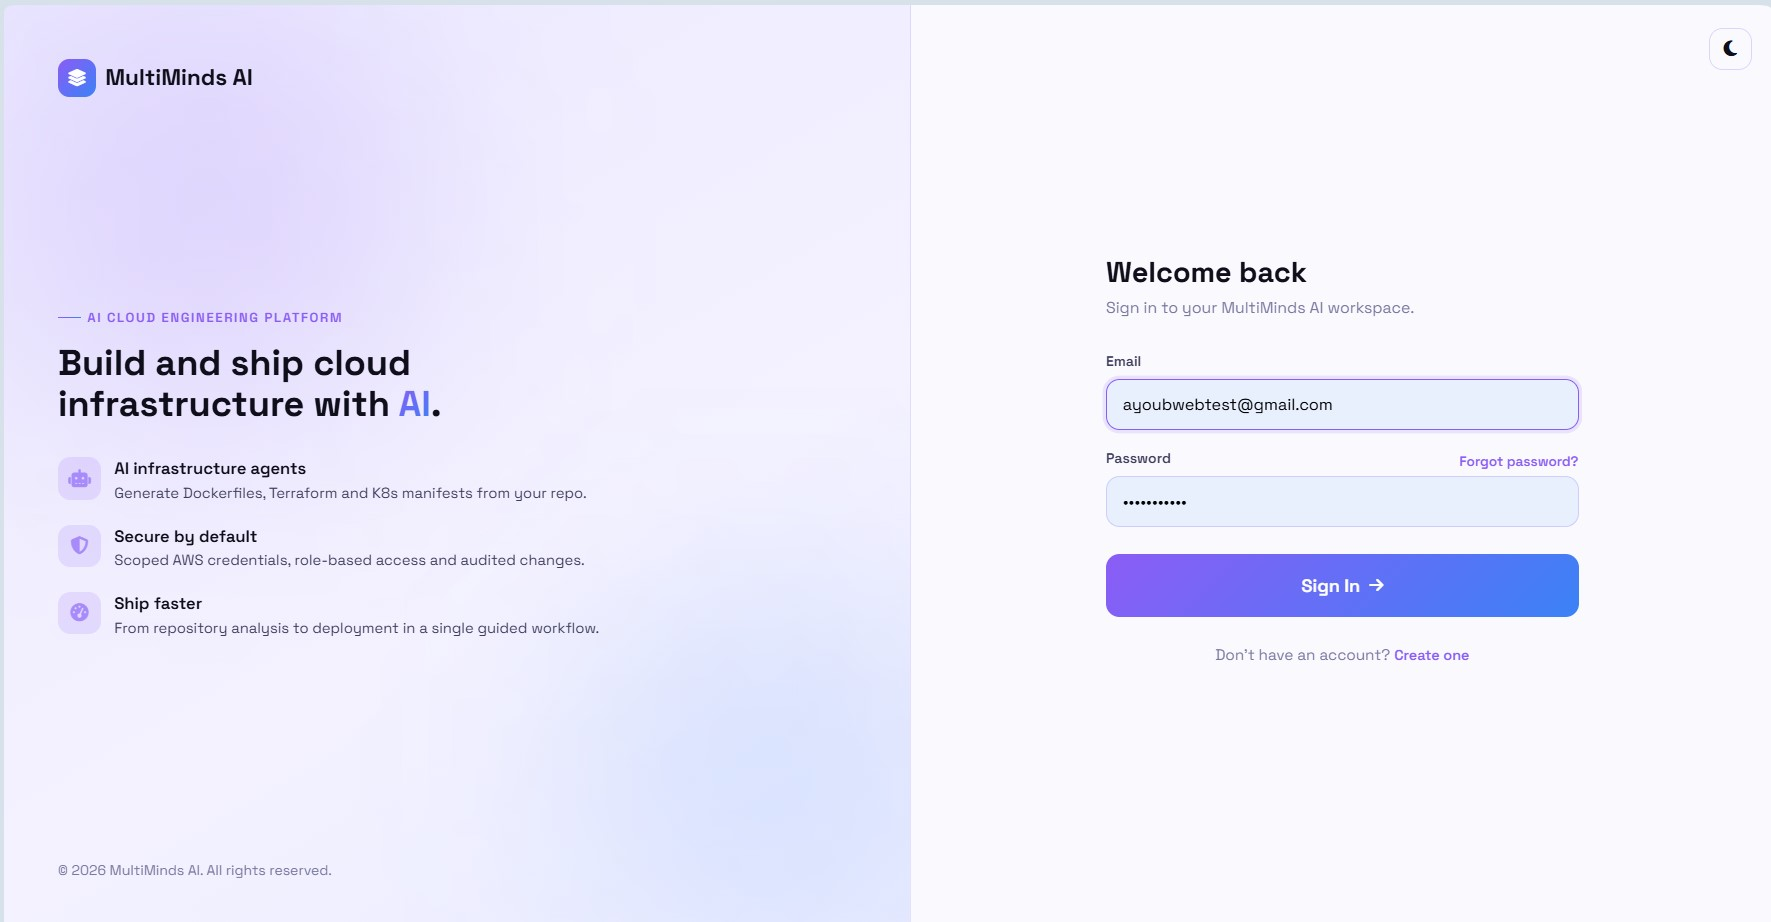
\includegraphics[width=0.75\textwidth]{images/Sign_in_page.jpg}
    \caption{Page d'authentification}
    \label{fig:sign-in}
\end{figure}

La figure~\ref{fig:sign-in} présente l'interface de connexion. L'utilisateur s'authentifie
à l'aide de ses identifiants pour accéder à son espace de travail et à ses projets.

\begin{figure}[H]
    \centering
    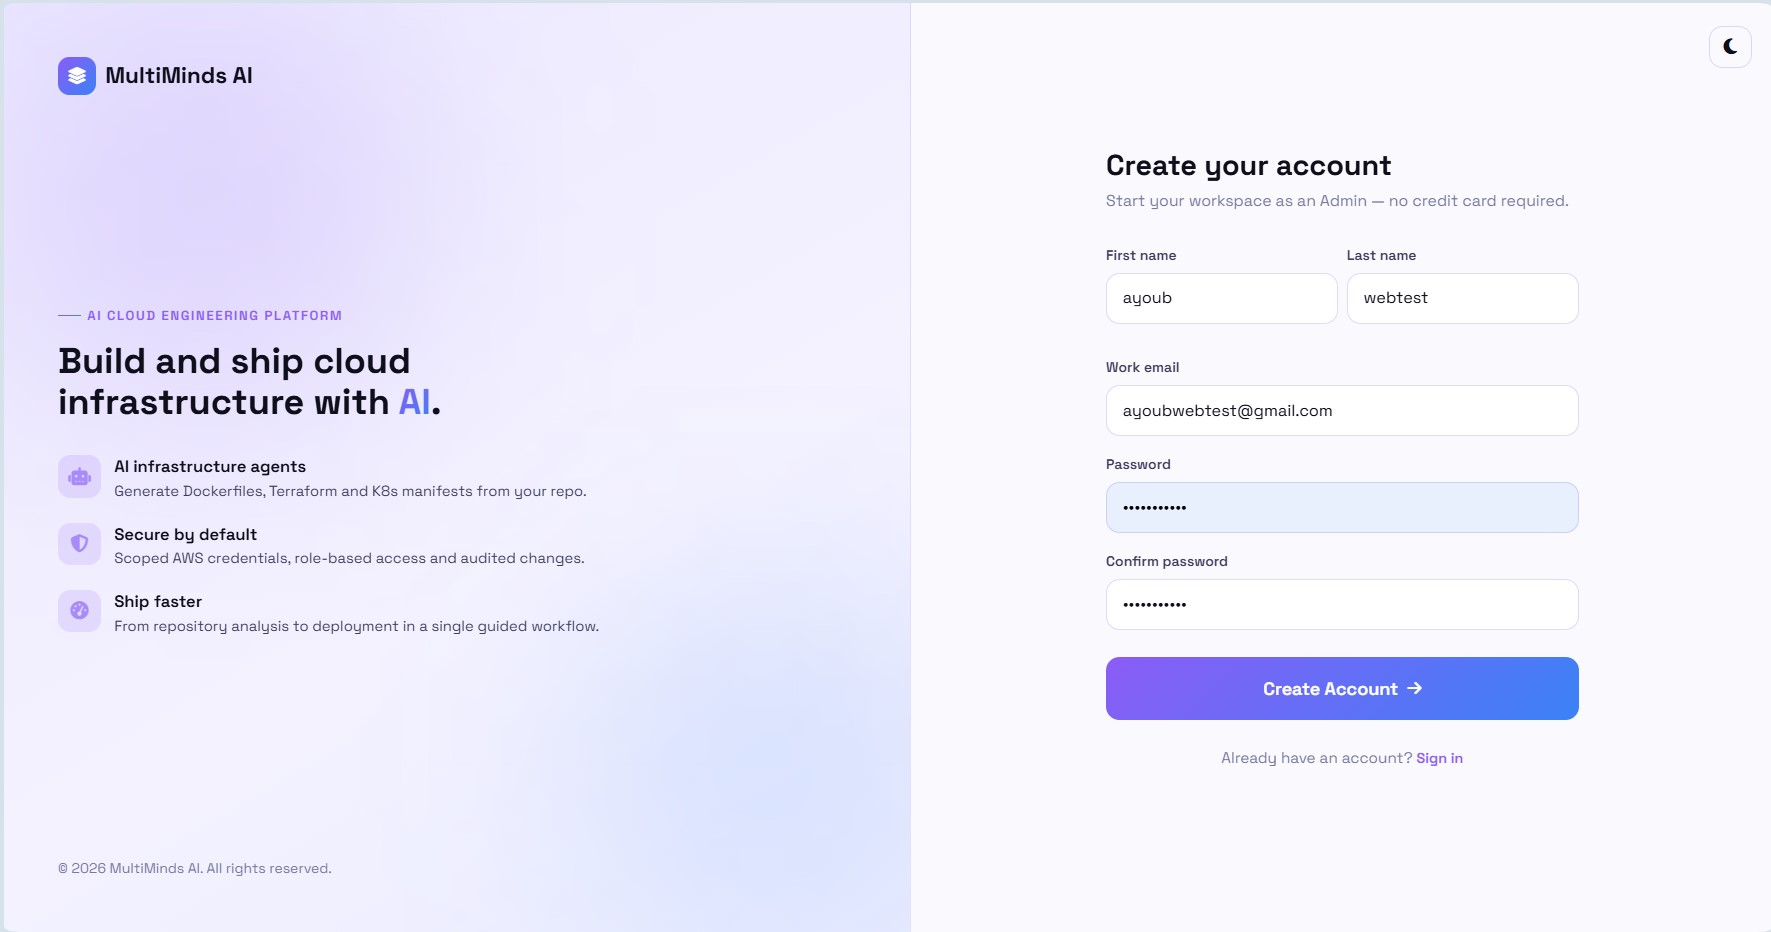
\includegraphics[width=0.75\textwidth]{images/Sign_up_page.jpg}
    \caption{Page d'inscription}
    \label{fig:sign-up}
\end{figure}

La figure~\ref{fig:sign-up} montre le formulaire de création de compte. Il permet à un
nouvel utilisateur de s'enregistrer avant de rejoindre ou de créer un espace de travail.

\begin{figure}[H]
    \centering
    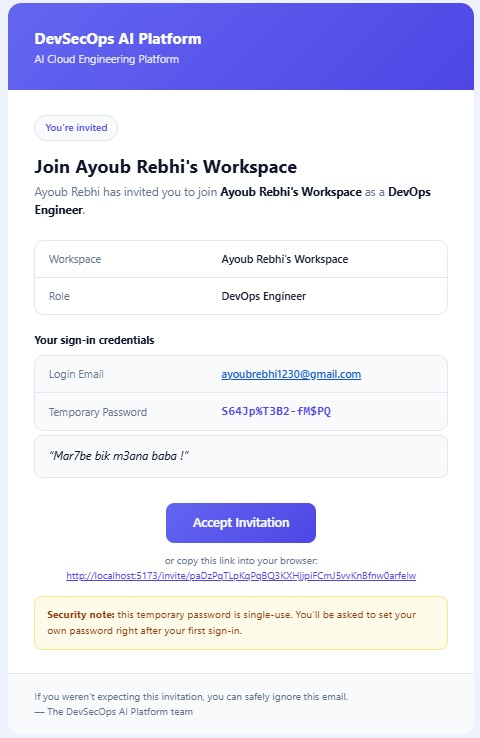
\includegraphics[width=0.75\textwidth]{images/invitation_mail.jpg}
    \caption{Courriel d'invitation}
    \label{fig:invitation-mail}
\end{figure}

La figure~\ref{fig:invitation-mail} illustre le courriel d'invitation envoyé
automatiquement à un membre. Il contient les informations d'accès nécessaires pour
rejoindre l'espace de travail.

\begin{figure}[H]
    \centering
    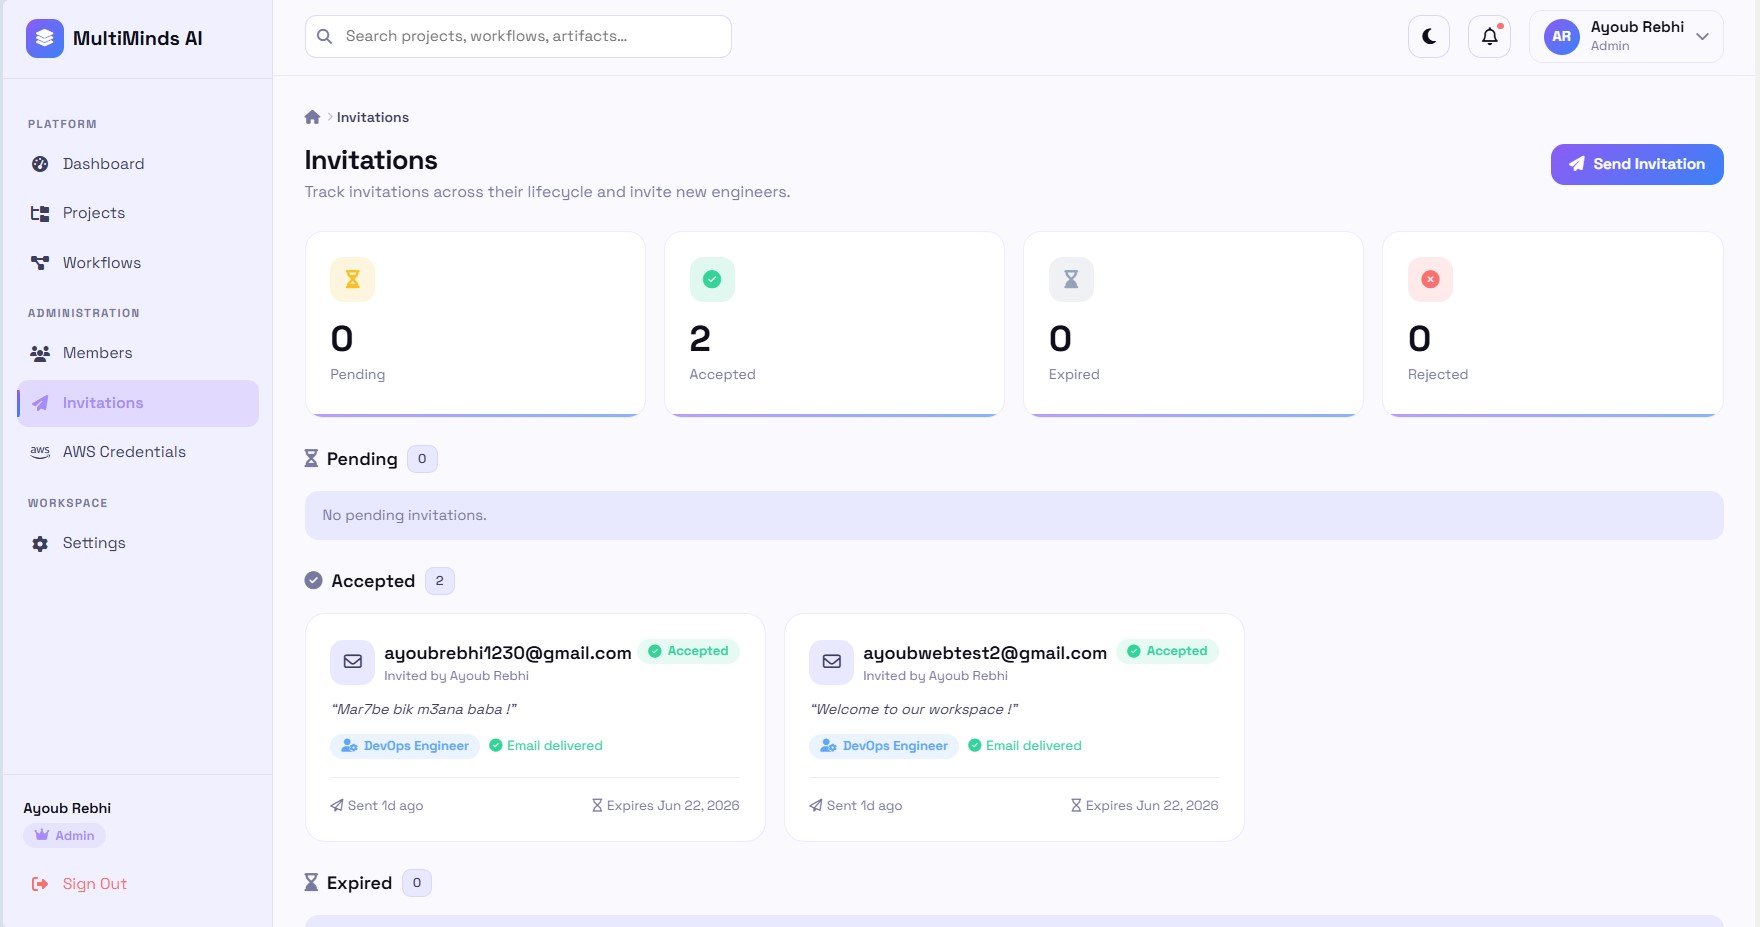
\includegraphics[width=0.85\textwidth]{images/Invite_members_to_workspace.jpg}
    \caption{Invitation de membres à l'espace de travail}
    \label{fig:invite-members}
\end{figure}

La figure~\ref{fig:invite-members} présente l'interface d'invitation des membres.
L'administrateur y ajoute de nouveaux collaborateurs et leur attribue un rôle.

\subsection{Tableau de bord et gestion des projets}

Le tableau de bord offre une vue d'ensemble de l'activité et donne accès à l'analyse
détaillée de chaque projet.

\begin{figure}[H]
    \centering
    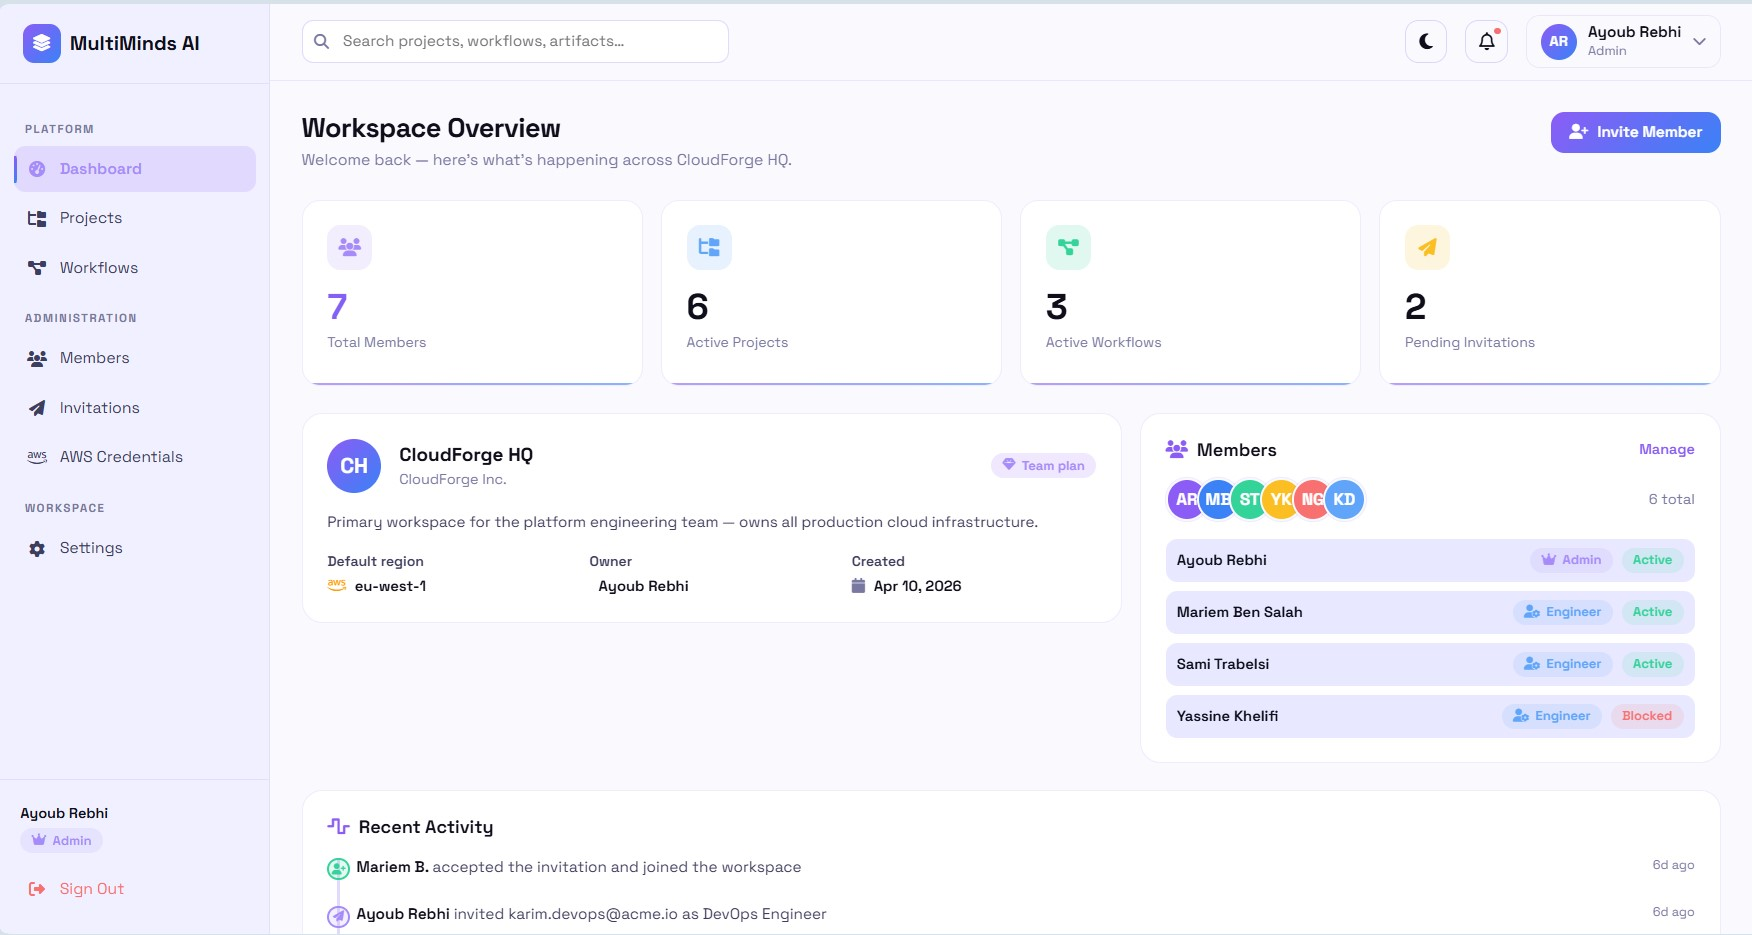
\includegraphics[width=0.9\textwidth]{images/Dashboard_admin.jpg}
    \caption{Tableau de bord administrateur}
    \label{fig:dashboard-admin}
\end{figure}

La figure~\ref{fig:dashboard-admin} présente le tableau de bord de l'administrateur. Il
synthétise l'état des projets, des workflows et des ressources gérées par la plateforme.

\begin{figure}[H]
    \centering
    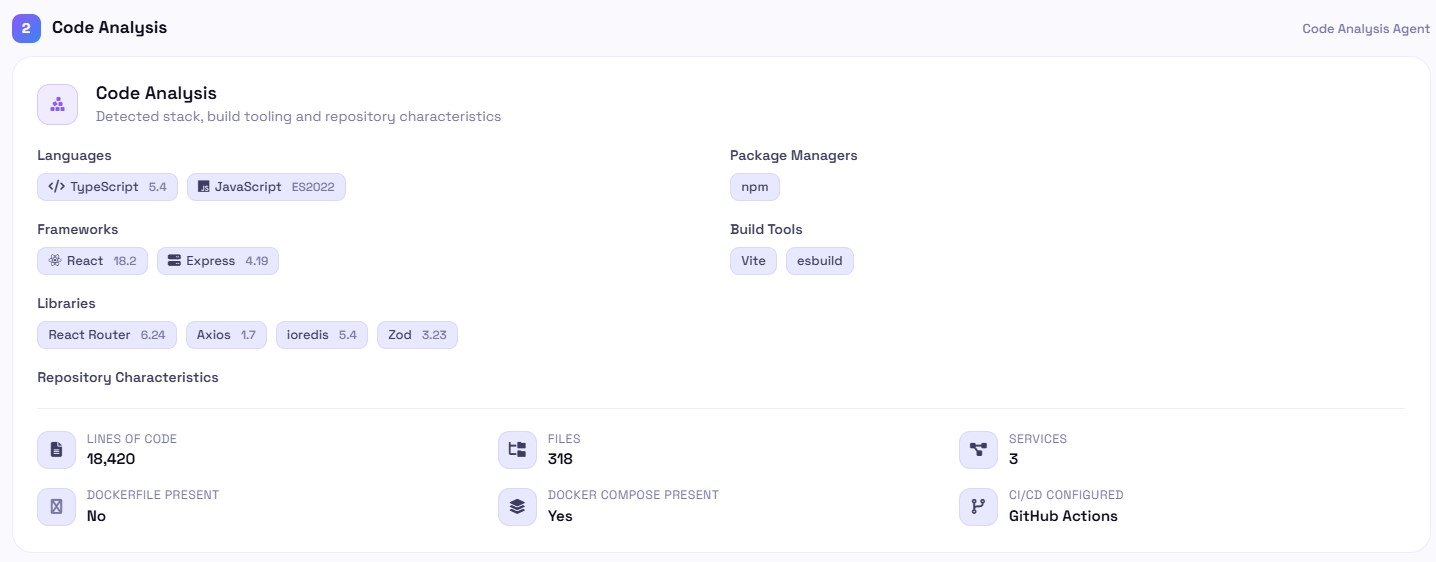
\includegraphics[width=0.9\textwidth]{images/Project_Analysis.jpg}
    \caption{Analyse d'un projet}
    \label{fig:project-analysis}
\end{figure}

La figure~\ref{fig:project-analysis} montre le résultat de l'analyse automatique d'un
projet. La plateforme identifie le langage, le framework et les dépendances afin de
guider les étapes suivantes du workflow.

\subsection{Sélection des architectures cloud}

À partir de l'analyse du projet, la plateforme propose plusieurs stratégies
d'architecture parmi lesquelles l'utilisateur effectue son choix.

\begin{figure}[H]
    \centering
    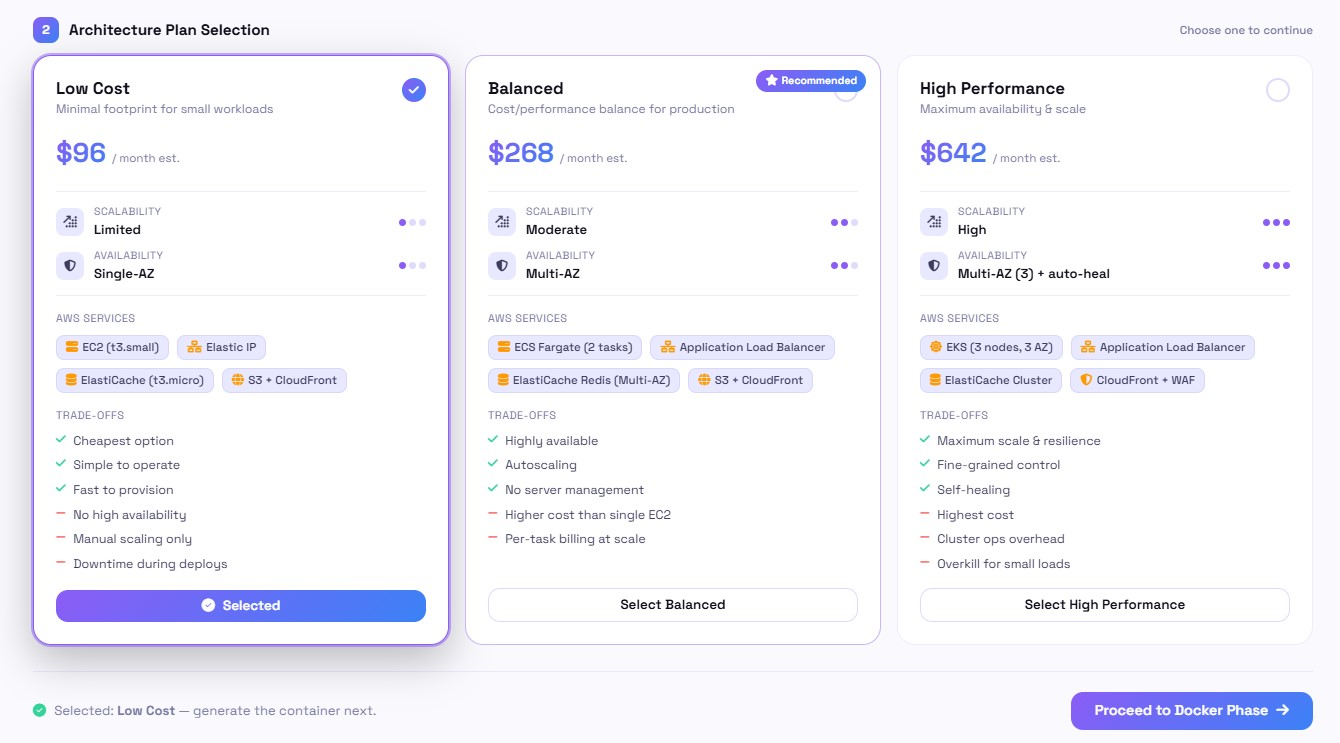
\includegraphics[width=0.9\textwidth]{images/Architecture plan selection.jpg}
    \caption{Sélection d'une architecture cloud}
    \label{fig:architecture-selection}
\end{figure}

La figure~\ref{fig:architecture-selection} présente les stratégies d'architecture
proposées (par exemple \textit{Low Cost}, \textit{Balanced}, \textit{High Performance}),
accompagnées d'une estimation de coût. L'utilisateur sélectionne l'option la mieux
adaptée à ses contraintes.

\subsection{Génération intelligente des artefacts DevOps}

La plateforme génère automatiquement les artefacts nécessaires au déploiement~:
Dockerfile, fichiers Terraform et pipelines CI/CD.

\begin{figure}[H]
    \centering
    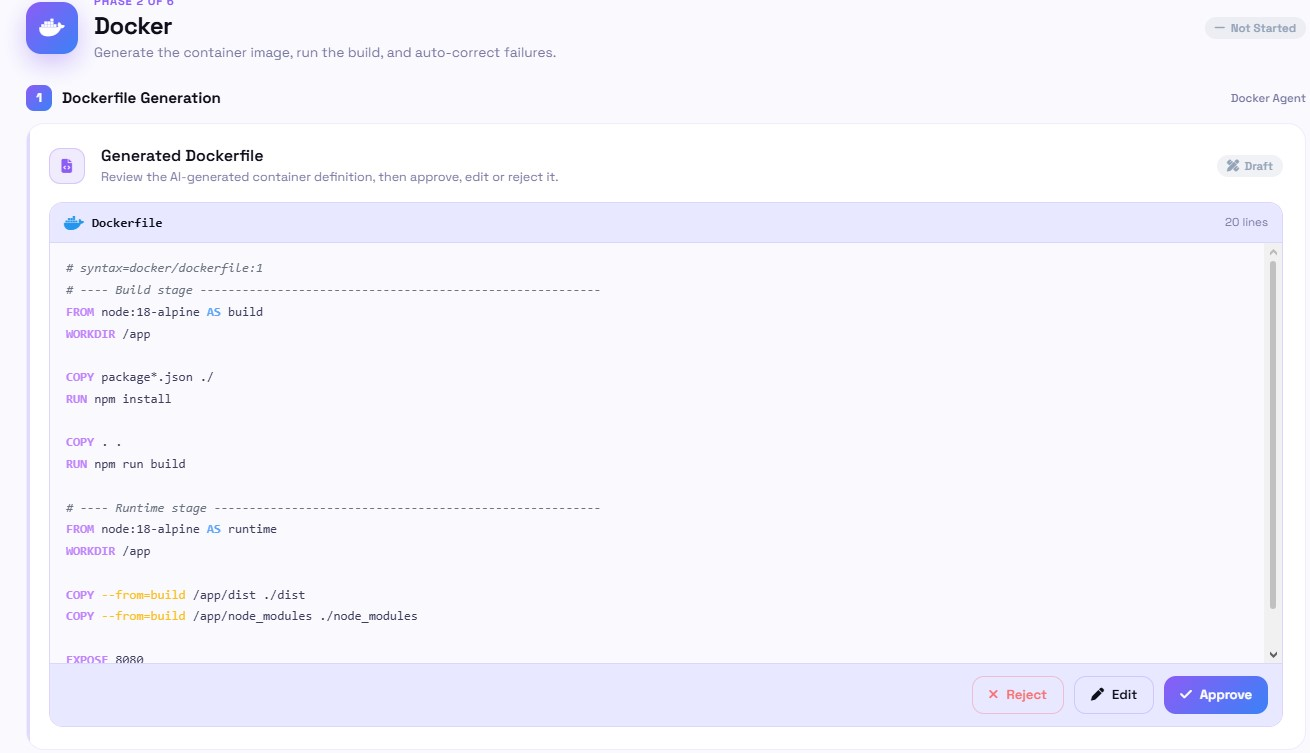
\includegraphics[width=0.9\textwidth]{images/Docker generation.jpg}
    \caption{Génération du Dockerfile}
    \label{fig:docker-generation}
\end{figure}

La figure~\ref{fig:docker-generation} illustre la génération d'un Dockerfile adapté au
projet, tenant compte du langage et des bonnes pratiques de sécurité et d'optimisation.

\begin{figure}[H]
    \centering
    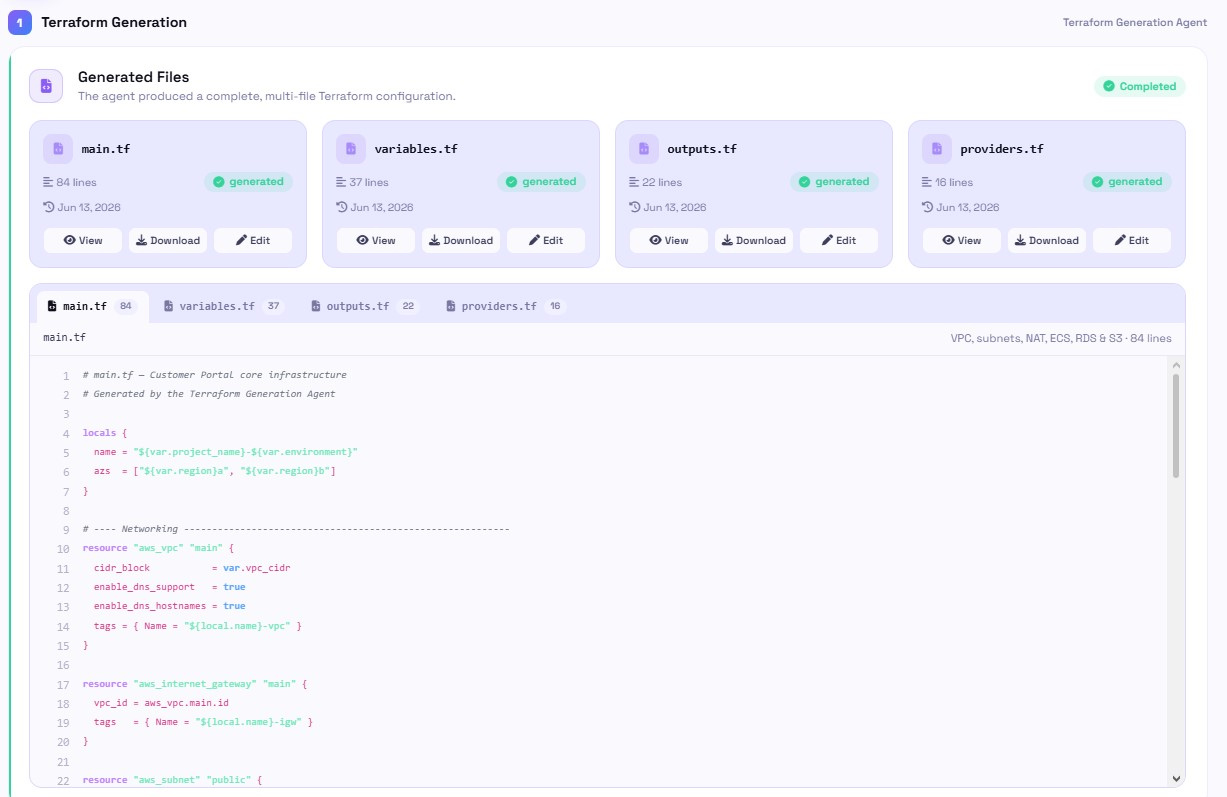
\includegraphics[width=0.9\textwidth]{images/TF Generation.jpg}
    \caption{Génération des fichiers Terraform}
    \label{fig:tf-generation}
\end{figure}

La figure~\ref{fig:tf-generation} montre la génération des fichiers Terraform
correspondant à l'architecture retenue, dans le respect des conventions HCL.

\begin{figure}[H]
    \centering
    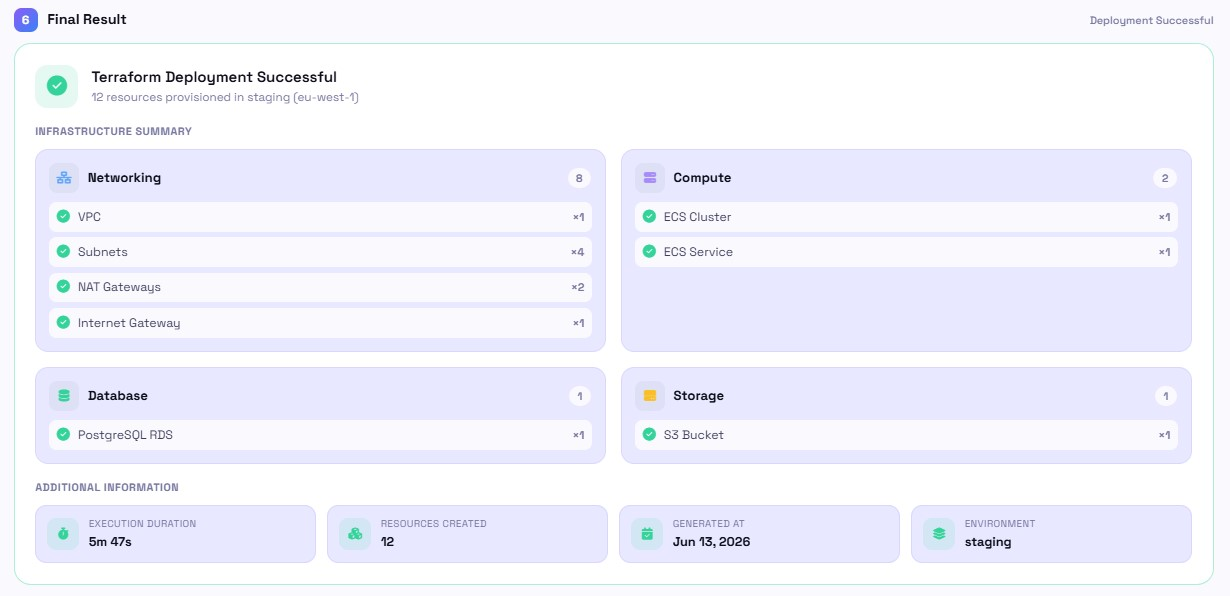
\includegraphics[width=0.9\textwidth]{images/final tf result.jpg}
    \caption{Résultat final de la génération Terraform}
    \label{fig:tf-final}
\end{figure}

La figure~\ref{fig:tf-final} présente les fichiers Terraform finalisés. Les ressources
déclarées sont cohérentes et prêtes à être validées puis planifiées.

\begin{figure}[H]
    \centering
    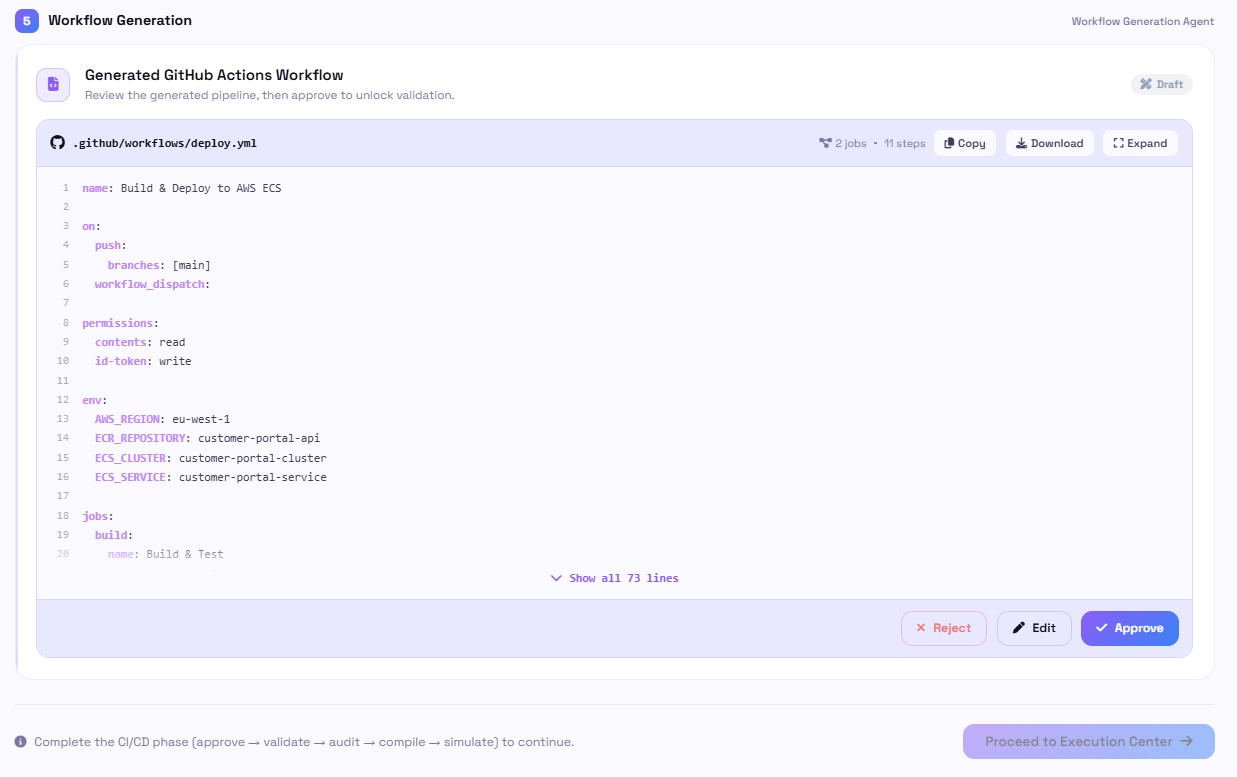
\includegraphics[width=0.9\textwidth]{images/Generated Github Action workflow.jpg}
    \caption{Workflow GitHub Actions généré}
    \label{fig:github-action}
\end{figure}

La figure~\ref{fig:github-action} illustre le pipeline GitHub Actions généré
automatiquement, intégrant les étapes de build, de test et de déploiement.

\subsection{Remédiation intelligente des erreurs}

En cas d'échec, le \textit{Corrector Agent} diagnostique l'erreur et propose une
correction soumise à la validation de l'utilisateur.

\begin{figure}[H]
    \centering
    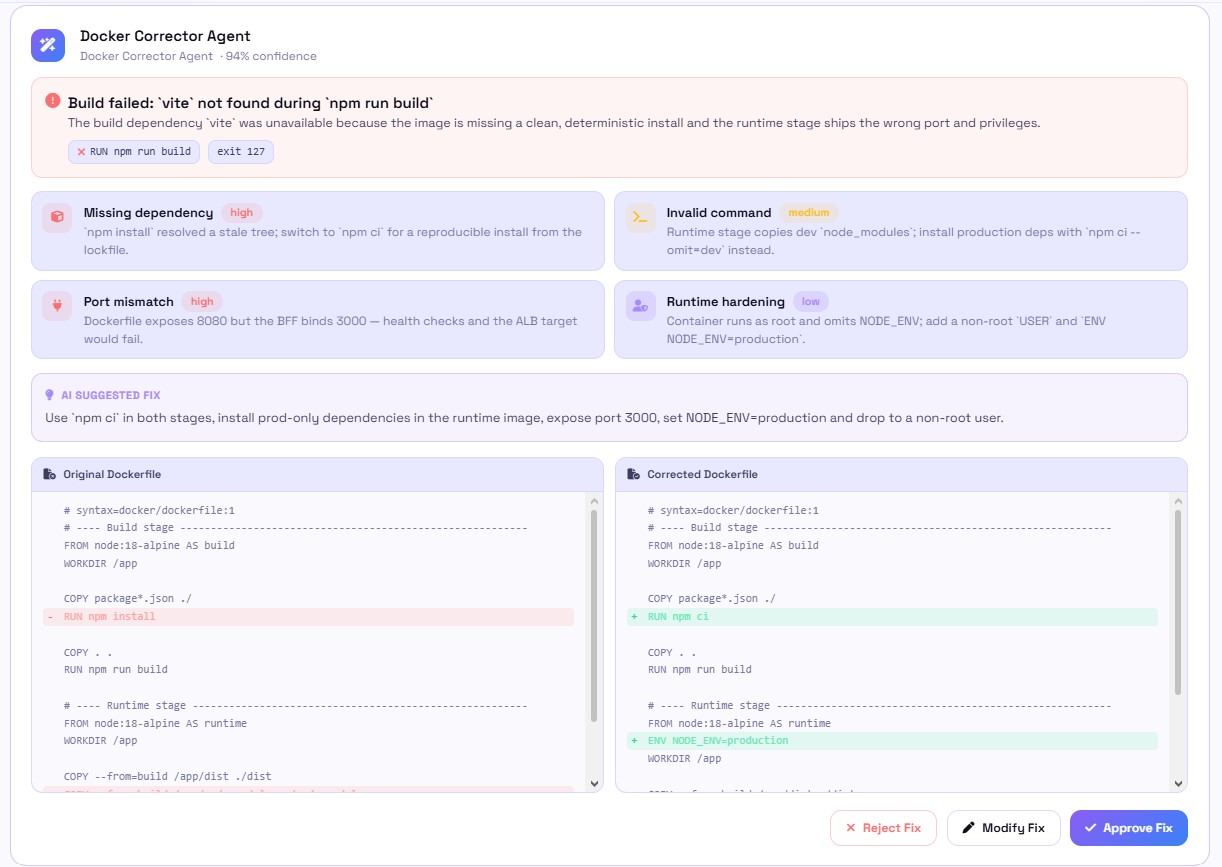
\includegraphics[width=0.9\textwidth]{images/Docker corrector agent.jpg}
    \caption{Correction assistée d'un Dockerfile}
    \label{fig:docker-corrector}
\end{figure}

La figure~\ref{fig:docker-corrector} montre le \textit{Corrector Agent} en action. À la
suite d'un échec de build, il analyse les journaux et propose une correction ciblée.

\begin{figure}[H]
    \centering
    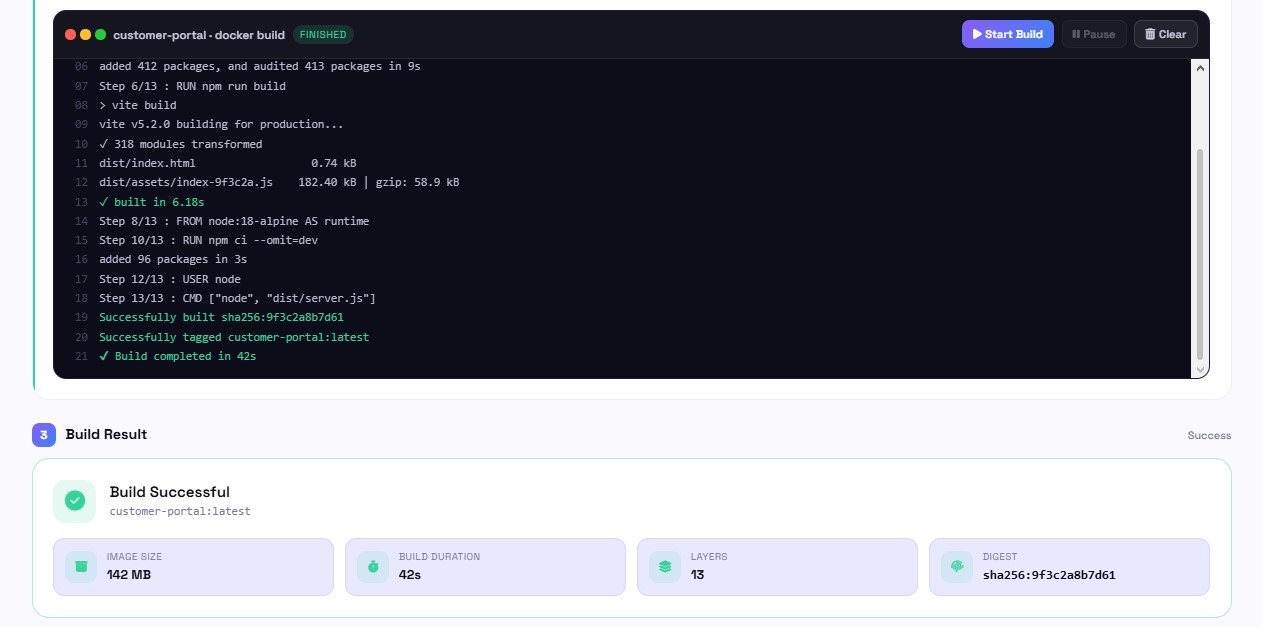
\includegraphics[width=0.9\textwidth]{images/Successfull docker build.jpg}
    \caption{Build Docker réussi après correction}
    \label{fig:docker-build-success}
\end{figure}

La figure~\ref{fig:docker-build-success} présente le résultat d'un build réussi après
application de la correction proposée, confirmant l'efficacité de la boucle de
remédiation.

\subsection{Validation et exécution des workflows}

La plateforme valide et exécute les artefacts générés tout en vérifiant leur conformité
et le respect des bonnes pratiques.

\begin{figure}[H]
    \centering
    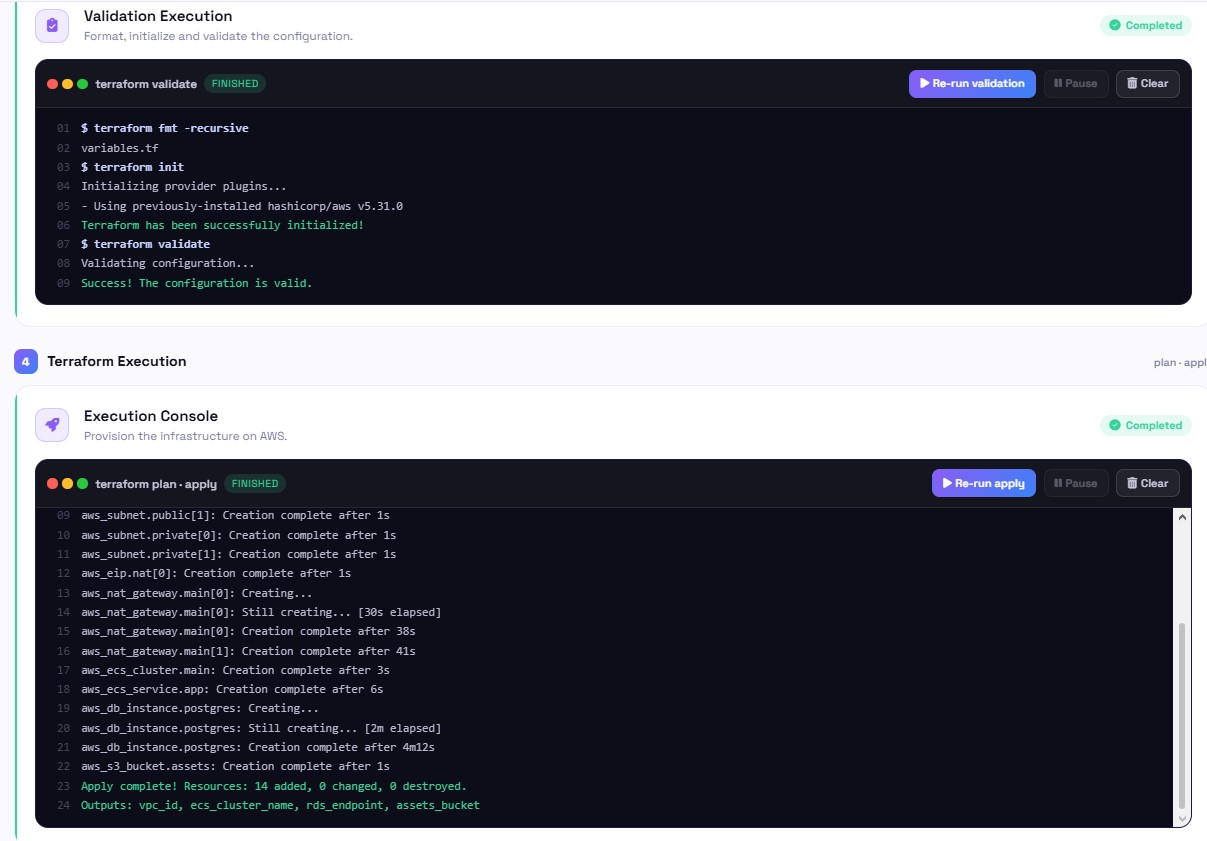
\includegraphics[width=0.9\textwidth]{images/tf execution success.jpg}
    \caption{Exécution Terraform réussie}
    \label{fig:tf-execution}
\end{figure}

La figure~\ref{fig:tf-execution} montre l'exécution réussie d'un plan Terraform. Les
ressources cloud sont provisionnées conformément à l'architecture sélectionnée.

\begin{figure}[H]
    \centering
    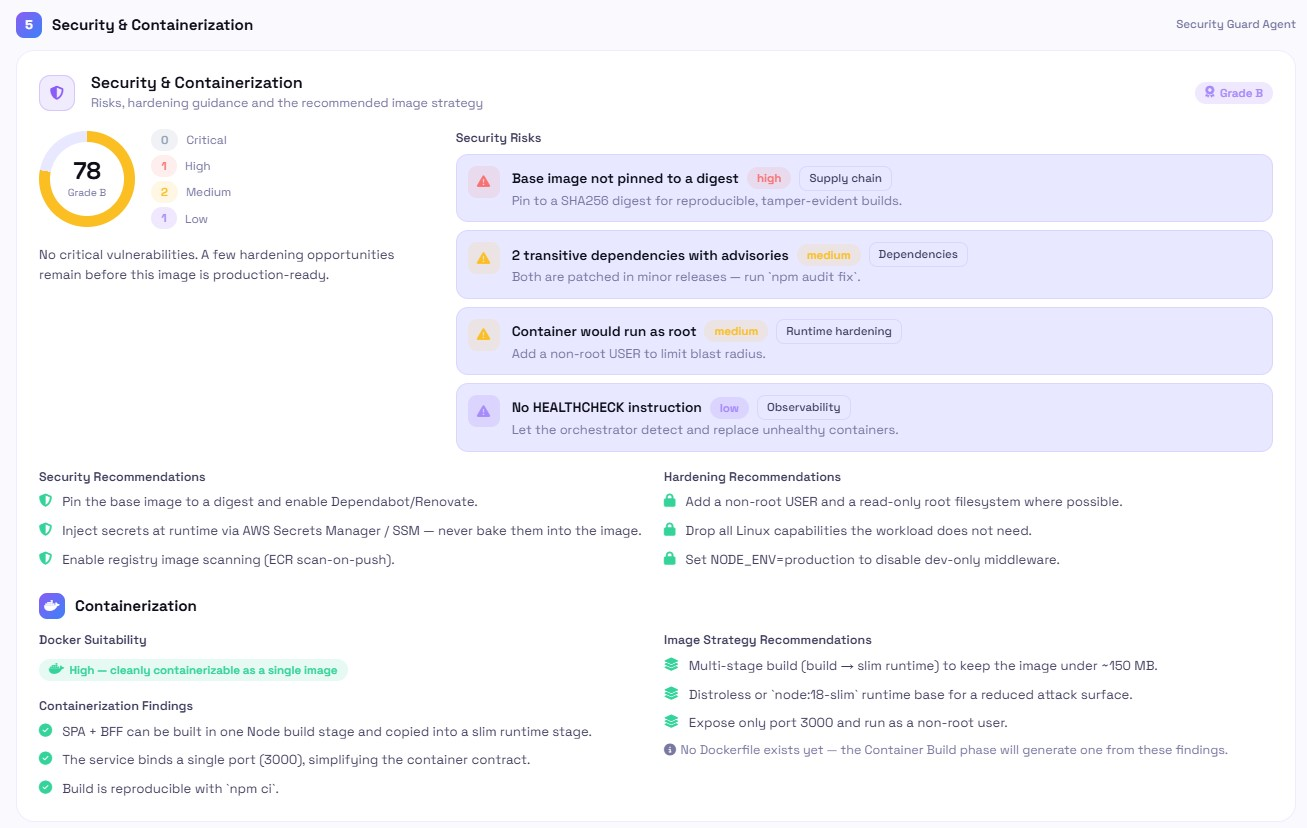
\includegraphics[width=0.9\textwidth]{images/Security agent.jpg}
    \caption{Vérification des bonnes pratiques dans les artefacts générés}
    \label{fig:security-agent}
\end{figure}

La figure~\ref{fig:security-agent} illustre la vérification des bonnes pratiques appliquée
aux artefacts générés. La sécurité y est traitée comme une exigence de qualité
transversale~: le contrôle vérifie que les artefacts respectent les bonnes pratiques
(utilisateur non-\textit{root}, permissions minimales, absence de secrets en clair) dès
leur génération, sans constituer une étape de sécurité isolée.

\section{Conclusion}

Ce chapitre a présenté la réalisation concrète de la plateforme. Nous avons d'abord
détaillé l'environnement de développement et les technologies retenues, puis illustré les
principales interfaces homme-machine couvrant l'authentification, la gestion des projets,
la sélection d'architecture et la génération des artefacts DevOps. Nous avons enfin validé
les capacités intelligentes du système~: la génération d'infrastructure cloud,
l'automatisation des pipelines CI/CD et la remédiation intelligente des erreurs.
L'ensemble confirme que la solution réalisée répond aux besoins exprimés et met
effectivement en œuvre les choix de conception définis précédemment.
